\chapter{Краткий обзор дифракции на кристаллах}
В это главе мы кратко дадим основные результаты кинетической и динамической теории дифракции. Основные кристаллы используемы на синхротронных источниках третьего и четвёртого поколений - это $Si$ (кремний), $C$ (алмаз) и реже $Ge$ (германий), в виду свой кубической кристаллический решётки, эти кристаллы относительно просты для анализа. Для нас важны такие свойства кристаллов, как способность преобразовать относительно широкой спектр излучения ондулятора, в излучение с относительной монохроматичностью до $\Delta E/ E \sim 10^{-4}$, а также поглощательные способности кристаллов, что в значительной степени снижает тепловые нагрузки на оптические элементы.
\section{Симметричное брэгговское отражение от идеально кристалла}
Длины волн, которые отвечают резонансу при отражении падающего под углом $\theta$ к плоскости кристалла излучения, даётся законом Брэгга:  
%пропорциональный $\gamma / nN$, где $n$ --- номер гармоники излучения, $N$ --- число периодов ондулятора, а $\gamma$ --- гамма фактор релятивистского электрона
\begin{equation}
	m\lambda = 2d\sin\theta,
\end{equation}
где $d$ --- расстояние между плоскостями от которых происходит отражение, а $m$ --- некоторое положительно целое число. Основной результат, который мы будем использовать, это кривая Дарвина, которая определяет угловой акцептанс излучения. Динамическая и кинематическая теории дифракции дают конечную ширину в, которую кристалл может принять излучение, а также некоторый сдвиг, относительно предполагаемого брэгговского угла. На рис.~\ref{fig:bragg_R} показаны характерные кривые отражение. По ним видно, что чем больше энергия подающего пучка излучения, тем уже кривая и ближе к даваемому законом брэгга углу. При расчёте кристаллов монохроматоров этот факт необходимо учитывать, так как излучение не попавшее в акцептанс кристалла будет поглощаться и выделять в нем тепло. 
\section{Поглощательные способности кристаллов}
Одним из полезных применение кристаллов в рентгеновском диапазоне есть их фильтрующая способность, отрезать низкие энергии, в особенности для алмазных кристаллов, которые, по мимо всего, имеют хорошую теплопроводность, что способствуют быстрому теплоотводу. На рис.~\ref{fig:bragg_T} представлена кривая поглощения 100 мкм кристалла алмаза. Подобные кристаллы устанавливают перед первыми оптическими элементами, что в значительной степени снижает тепловые нагрузки, подавлением низших гармоник.
\begin{figure}
	\centering  
	\begin{minipage}{0.49\textwidth}
		\centering
		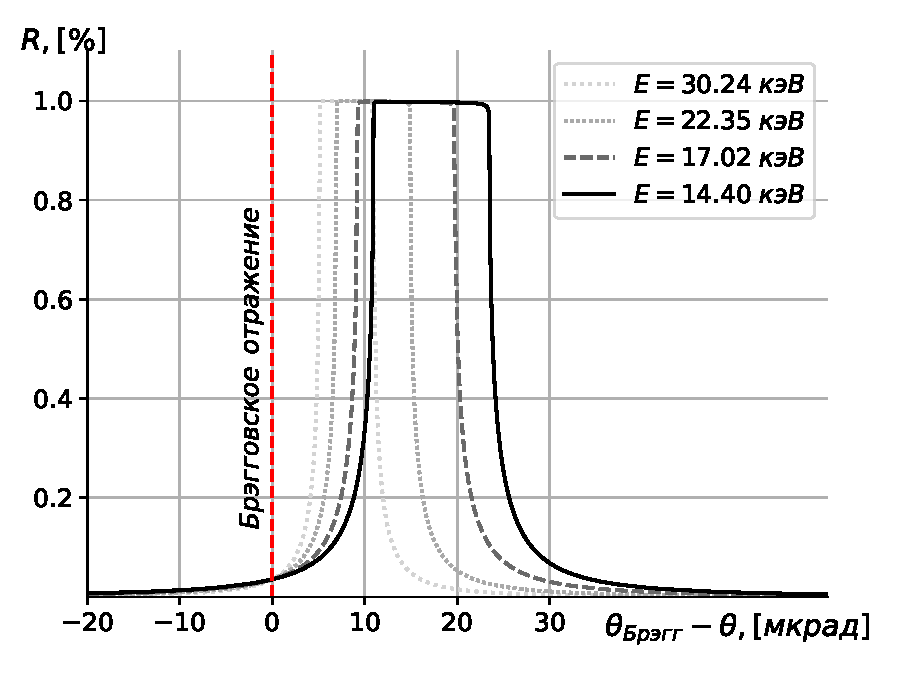
\includegraphics[width=\textwidth]{pic/bragg_R.pdf}
		\caption{}
		\label{fig:bragg_R}
	\end{minipage}\hfill
	\begin{minipage}{0.49\textwidth}
		\centering
		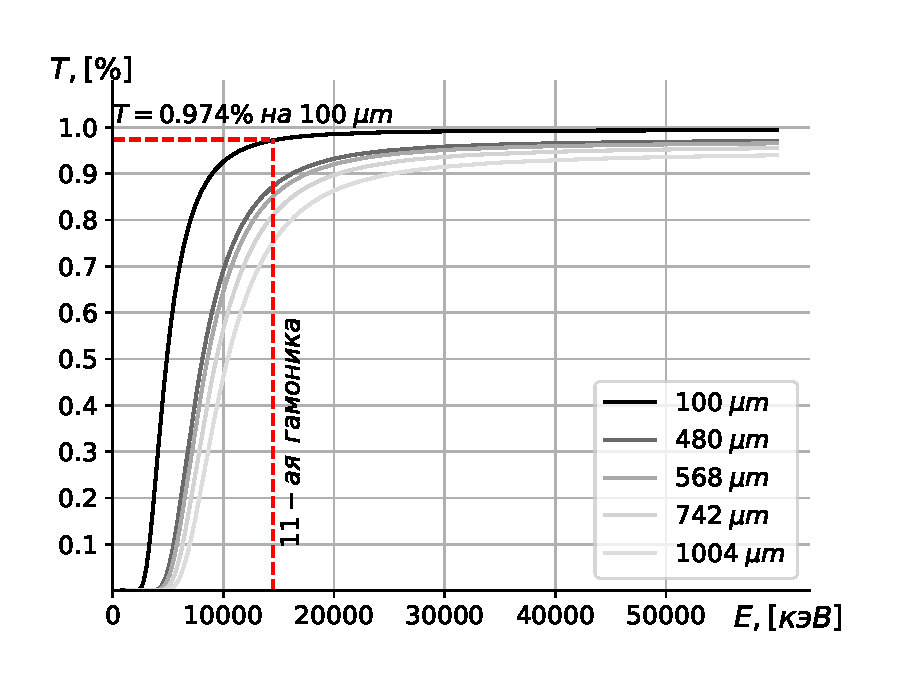
\includegraphics[width=\textwidth]{pic/bragg_T.pdf}
		\caption{}
		\label{fig:bragg_T}
	\end{minipage}    
\end{figure}
